% ICRA template
% Obtained from 
% Modified for the purposes of this tutorial

%%%%%%%%%%%%%%%%%%%%%%%%%%%%%%%%%%%%%%%%%%%%%%%%%%%%%%%%%%%%%%%%%%%%%%%%%%%%%%%%
% IEEE setup
\documentclass[letterpaper, 10 pt, conference]{ieeeconf}  % Comment this line out if you need a4paper
%\documentclass[a4paper, 10pt, conference]{ieeeconf}      % Use this line for a4 paper

\IEEEoverridecommandlockouts                              % This command is only needed if 
                                                          % you want to use the \thanks command

\overrideIEEEmargins                                      % Needed to meet printer requirements.

%%%%%%%%%%%%%%%%%%%%%%%%%%%%%%%%%%%%%%%%%%%%%%%%%%%%%%%%%%%%%%%%%%%%%%%%%%%%%%%%
% Additional packages
\usepackage{lipsum}             % To fill blocks of text with lorem ipsum
\usepackage{balance}            % This levels the references at the end of the document

\setlength {\marginparwidth }{2cm}
\usepackage{todonotes}          % To add TODOs and missingfigures

\usepackage[dvipsnames]{xcolor} % Named colours (the default ones are boring) https://www.overleaf.com/learn/latex/Using_colors_in_LaTeX#Accessing_additional_named_colors

\usepackage{hyperref}           % To enable links and colour them

% The setup below is to colourise the links using the xcolor colours
\hypersetup{
    colorlinks=true      % to enable colour in the links
    ,linkcolor=NavyBlue
    ,citecolor=red
    ,filecolor=NavyBlue
    ,urlcolor= NavyBlue
    ,menucolor=NavyBlue
    ,runcolor=NavyBlue
    ,linkbordercolor=NavyBlue
    ,citebordercolor=NavyBlue
    ,filebordercolor=NavyBlue
    ,urlbordercolor=NavyBlue
    ,menubordercolor=NavyBlue
    ,runbordercolor=NavyBlue
}

\usepackage{siunitx}            % To have standard SI units

% The settings below make sure the units look the same as the text style
\sisetup{per-mode = symbol,
         detect-weight = true,
         range-phrase = --,
         range-units = single,
         detect-all = true}

% The packages below are required for the front-page double-column hero figure
\usepackage{caption}            % To create captions for the hero figure
\captionsetup[figure]{font=footnotesize,labelfont=footnotesize} % this is to make them comply with the IEEE template
 

%%%%%%%%%%%%%%%%%%%%%%%%%%%%%%%%%%%%%%%%%%%%%%%%%%%%%%%%%%%%%%%%%%%%%%%%%%%%%%%%
% Document begins
\begin{document}

\title{\LARGE \bf
My Fake ICRA Submission for the Purposes of this Tutorial
}

\author{Mat{\'i}as Mattamala$^{1}$
}

%%%%%%%%%%%%%%%%%%%%%%%%%%%%%%%%%%%%%%%%%%%%%%%%%%%%%%%%%%%%%%%%%%%%%%%%%%%%%%%%
% Example of two-column hero figure
% This needs to go before the abstract!
% Please note that this is all needed to make it work

\twocolumn[{%
\renewcommand\twocolumn[1][]{#1}%
% In this case we need to add the title creation within this block
\maketitle
% Now we add the hero figure
\begin{center}
    \centering
    % Basic sketch
    \missingfigure{\textbf{Example of a basic sketch.} This figure should illustrate an example of what your paper is about. However, we use double column here to make it even more impressive.}
    % Caption
    \captionof{figure}{\textbf{A double-column hero figure.} Placing this figure here in the document is slightly more involved than standard figures, because we need to wrap it in a \texttt{twocolumn} environment, but if you check the source code you will get a good idea on how it is done.}
    \label{fig:hero-figure-double}
    \vspace{10pt}
\end{center}%
}]

\begingroup
  \renewcommand\thefootnote{}\footnote{
  $^{1}$The author is with the Oxford Robotics Institute, University of Oxford
  {\tt\small matias@robots.ox.ac.uk}
  }
  \addtocounter{footnote}{-1}%
\endgroup


%%%%%%%%%%%%%%%%%%%%%%%%%%%%%%%%%%%%%%%%%%%%%%%%%%%%%%%%%%%%%%%%%%%%%%%%%%%%%%%%
% Uncomment the following line if not using the hero figure
% \maketitle

\begin{abstract}
    This document has the purpose of supporting the graphics tutorial. This should illustrate how to make different things we might be interested in, such as hero figures, and figure sketches.
\end{abstract}

%%%%%%%%%%%%%%%%%%%%%%%%%%%%%%%%%%%%%%%%%%%%%%%%%%%%%%%%%%%%%%%%%%%%%%%%%%%%%%%%
\section{Introduction}
This document shows some examples to get properties of a \LaTeX document, which might be useful to design your graphics.

\section{Double-column Hero Figure}
Making a double-column hero or teaser figure requires a few hacks. In this document we have an example at the top of the front page. The code to generate it is:

\begin{footnotesize}
\begin{verbatim}
\twocolumn[{%
\renewcommand\twocolumn[1][]{#1}%
\maketitle
% Now we add the hero figure
\begin{center}
    \centering
    \missingfigure{\textbf{Basic sketch.} (...)}
    % Caption
    \captionof{figure}{\textbf{Caption} (...)}
    \label{fig:hero-figure-double}
\end{center}%
}]

\begingroup
    \renewcommand\thefootnote{}\footnote{
    $^{1}$The author is with (...)
    {\tt\small matias@robots.ox.ac.uk}
    }
    \addtocounter{footnote}{-1}%
\endgroup
\end{verbatim}
\end{footnotesize}

Please note here that we need to wrap the \texttt{maketitle} command within the block to make it work, so the title, authors, and figure are generated together before we start with the abstract and main text. This also requires to hack the \texttt{thanks} commands sometimes used in the ICRA template, and instead make it 'manually' as the bottom block shows.

\section{Getting the Text and Column Size}
When designing figures, we might want to know the \emph{real} size of the areas available on the paper. For that, we have a few commands to get the numbers directly.

\subsection{Text Size}
The \textbf{text size} corresponds to the full width of the 'writeable' area in the paper, i.e., both columns. To obtain it, in \emph{points}, we can use the command:

\begin{verbatim}
    \the\textwidth
\end{verbatim}
Which will output:
%
\begin{quotation}
\the\textwidth
\end{quotation}

\subsection{Column Size}
The \textbf{column size} is useful when we have double column papers, such as ICRA, IROS, RSS, or TRO. To obtain the size, we can use:
\begin{verbatim}
    \the\columnwidth
\end{verbatim}
which will output:
%
\begin{quotation}
\the\columnwidth
\end{quotation}

\subsection{Line Width}
The \textbf{line width} sets the size of a line of text. This will correspond to different measures depending on the document being single or double column. Similarly:
\begin{verbatim}
    \the\linewidth
\end{verbatim}
will output:
%
\begin{quotation}
    \the\linewidth
\end{quotation}

Just as a reminder, since these numbers are in \emph{points} (pt), you need to convert them to inches by dividing by $72.27$.

\section{Using SI Units}
To ensure that the units are used consistently across your paper, the \texttt{siunitx} package is very useful. It's a bit more verbose than writing the abbreviation yourself but it will guarantee that the format is consistent. For example, the following commands:

\begin{verbatim}
\SI{1}{\meter}
\SI{1}{\milli\meter}
\SI{10}{\degree}
\SI{30}{\hertz}
\end{verbatim}
will render:

\begin{quotation}
\noindent\SI{1}{\meter}\\
\SI{1}{\milli\meter}\\
\SI{10}{\degree}\\
\SI{30}{\hertz}\\
\end{quotation}

\section{Examples of Figures}
Next I show some examples of figures. I followed the same \emph{style} across them, using the same font and color palette.
I have also added fake text, just to distribute them better across the document and give you a sense on how to control where they are placed.


\subsection{Hero Figure}
{\color{gray}{\lipsum[1-5]}}
\begin{figure}[t]
    \centering
    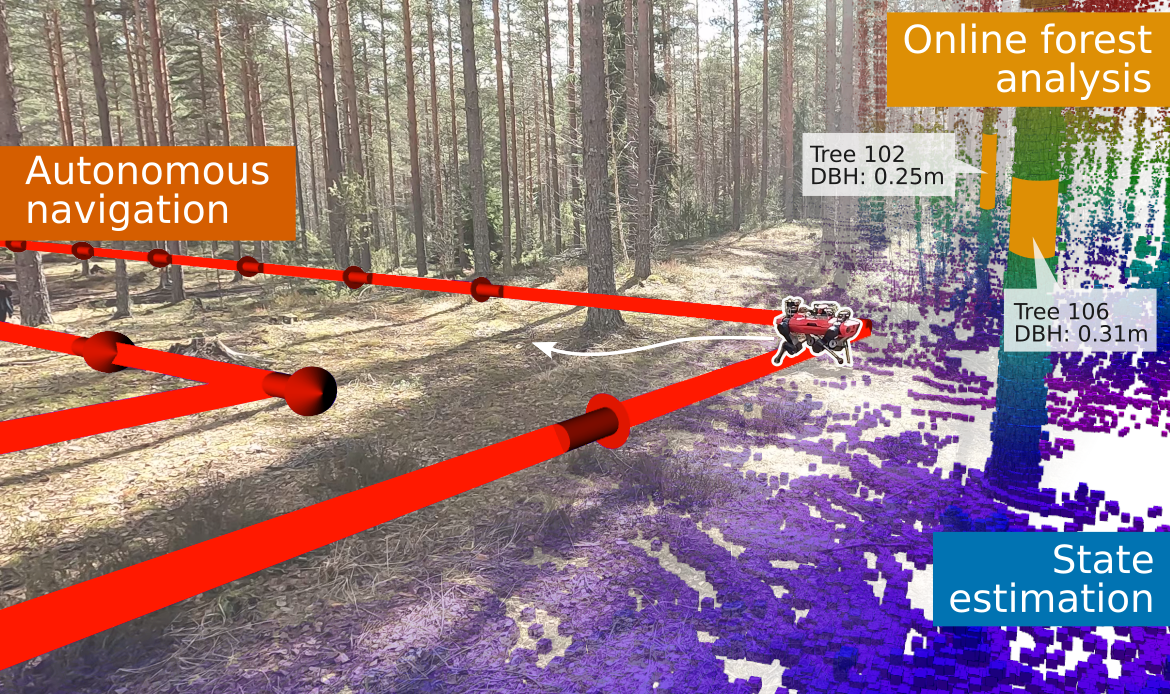
\includegraphics[width=\columnwidth]{figs/depiction.png}
    \caption{\textbf{A hero figure.}}
    \label{fig:hero-figure-single}
\end{figure}

\subsection{Systems Diagram Figure}
{\color{gray}{\lipsum[1-5]}}

\begin{figure}[t]
    \centering
    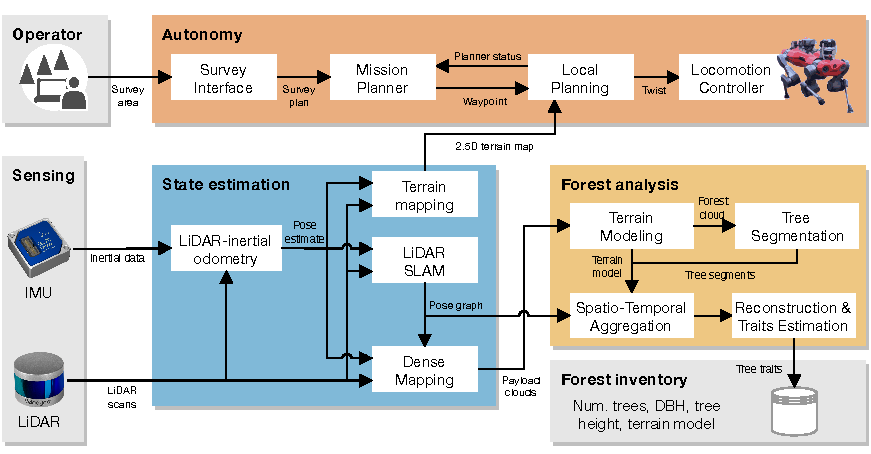
\includegraphics[width=\columnwidth]{figs/system_overview.pdf}
    \caption{\textbf{A systems figure.}}
    \label{fig:systems-figure-single}
\end{figure}

\subsection{Double column figure}
{\color{gray}{\lipsum[1-3]}}

\begin{figure*}[ht]
    \centering
    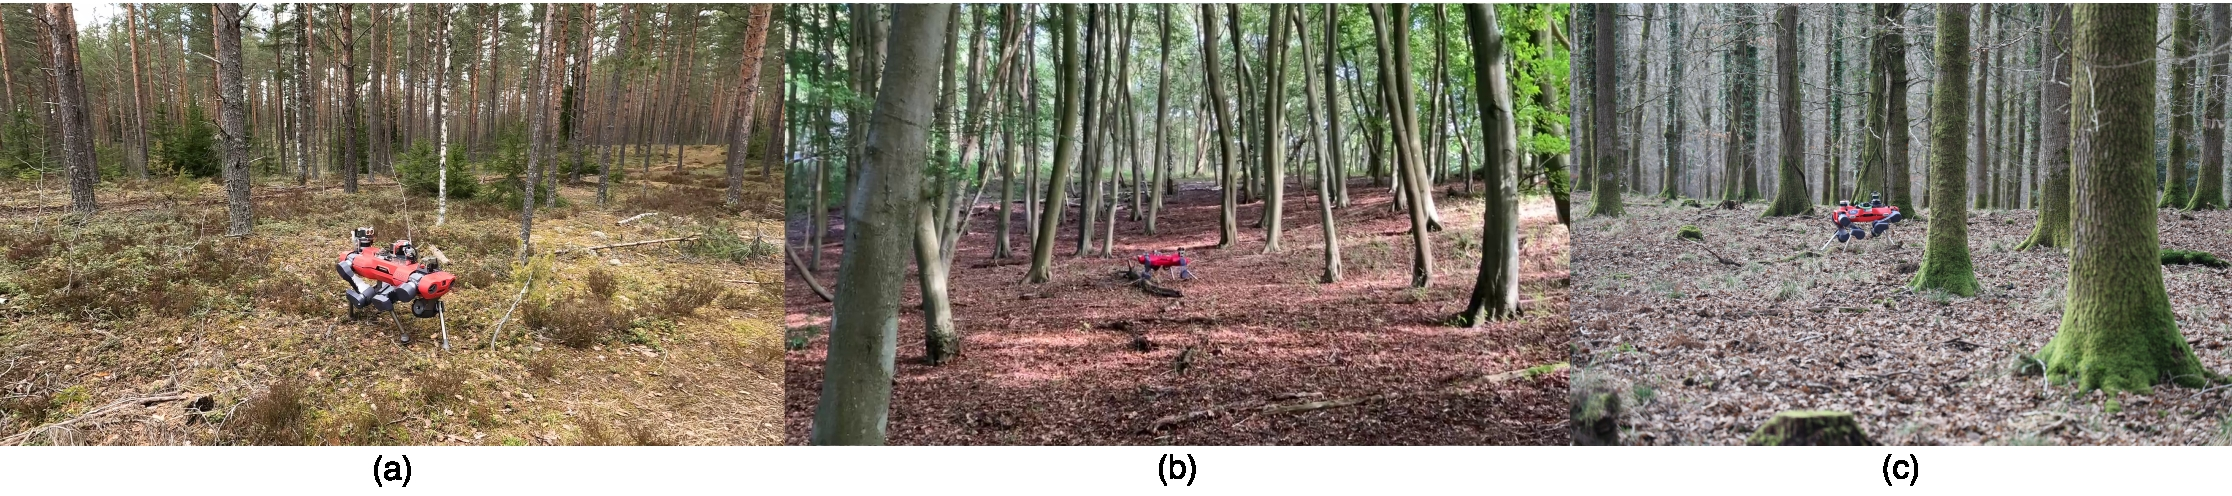
\includegraphics[width=\textwidth]{figs/deployments_ws.jpg}
    \caption{\textbf{Double column figure.} This is done with the \texttt{figure*} environment.}
    \label{fig:double-column}
\end{figure*}

{\color{gray}{\lipsum[1-3]}}


\subsection{Results Figure}
{\color{gray}{\lipsum[1-3]}}
\begin{figure}[b]
    \centering
    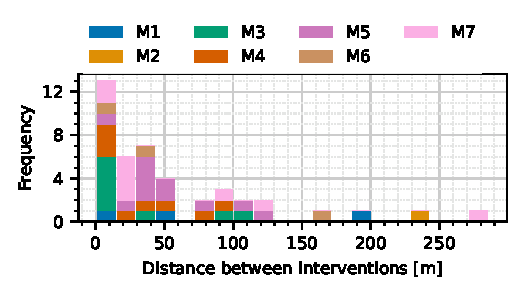
\includegraphics[width=\columnwidth]{figs/distance_between_interventions_distribution.pdf}
    \caption{\textbf{Single column Results Figure.} This is set to appear at the bottom.}
    \label{fig:double-column}
\end{figure}

{\color{gray}{\lipsum[1-3]}}


\section{Conclusions}

I hope this tutorial was useful.


%%%%%%%%%%%%%%%%%%%%%%%%%%%%%%%%%%%%%%%%%%%%%%%%%%%%%%%%%%%%%%%%%%%%%%%%%%%%%%%%
\section*{Appendix}

Not included any here.

\section*{Acknowledgment}

The author thanks Christina Kassab~\cite{kassab2025ol3d} and Ethan Tao~\cite{tao2022pdc} for providing figures and TeX examples from their prior papers for this tutorial.


%%%%%%%%%%%%%%%%%%%%%%%%%%%%%%%%%%%%%%%%%%%%%%%%%%%%%%%%%%%%%%%%%%%%%%%%%%%%%%%%

\balance

% ICRA
\bibliographystyle{IEEEtran}
\bibliography{references}

\end{document}
